\documentclass[twoside]{article}
\makeatletter
\def\input@path{{include/}}
\makeatother
\usepackage{aistats2026}

\usepackage{mathrsfs,amsmath,amsfonts,amssymb,bm,eufrak,pifont,amscd,euscript,amsthm,color,epsfig,xr,tikz,verbatim,enumitem}
\usepackage[utf8]{inputenc} % allow utf-8 input
\usepackage[T1]{fontenc}    % use 8-bit T1 fonts   % hyperlinks
\usepackage{url}            % simple URL typesetting
\usepackage{booktabs}       % professional-quality tables
\usepackage{flafter}        % keep floats after their definition
\usepackage{nicefrac}       % compact symbols for 1/2, etc.
\usepackage{microtype}      % microtypography
\usepackage{xcolor}
\usepackage{hyperref}  
% \usepackage{amssymb}
\usepackage{cleveref}
\usepackage{graphicx}
\usepackage{array}
\usepackage{subcaption}
\usepackage[round]{natbib}
\usepackage{wrapfig}
% \usepackage{include/titletoc}
\usepackage[makeroom]{cancel}
% \usepackage{caption}
\newcommand{\tarc}{\mbox{$\frown$}}
\newcommand{\arc}[1]{\stackrel{\raisebox{-0.5ex}{\tarc}}{#1}}

\allowdisplaybreaks
\usetikzlibrary{decorations.markings}

\definecolor{mydarkblue}{rgb}{0,0.08,0.45}

\hypersetup{ %
    pdftitle={},
    pdfauthor={},
    pdfsubject={},
    pdfkeywords={},
    pdfborder=0 0 0,
    pdfpagemode=UseNone,
    colorlinks=true,
    linkcolor=mydarkblue,
    citecolor=mydarkblue,
    filecolor=mydarkblue,
    urlcolor=mydarkblue,
    pdfview=FitH
}

\newtheorem{assumption}{Assumption}
\Crefname{assumption}{Assumption}{Assumption} 
\crefname{assumption}{Assumption}{Assumption} 

\usepackage{aliascnt}

\newenvironment{talign*}
 {\let\displaystyle\textstyle\csname align*\endcsname}
 {\endalign}
\newenvironment{talign}
 {\let\displaystyle\textstyle\csname align\endcsname}
 {\endalign}


\usepackage{tikz}
\usetikzlibrary{calc}
\usepackage[title]{appendix}


\newtheorem{theorem}{Theorem}[section]
\crefname{theorem}{Theorem}{Theorems}
\Crefname{theorem}{Theorem}{Theorems}
\newaliascnt{lem}{theorem}
\newtheorem{lem}[lem]{Lemma}
\aliascntresetthe{lem}
\crefname{lem}{Lemma}{Lemmas}
\Crefname{lem}{Lemma}{Lemmas}

\newaliascnt{prop}{theorem}
\newtheorem{prop}[prop]{Proposition} 
\aliascntresetthe{prop}
\crefname{prop}{Proposition}{Propositions}
\Crefname{prop}{Proposition}{Propositions}

\newtheorem{ass}{Assumption}
\crefname{ass}{Assumption}{Assumptions}
\Crefname{ass}{Assumption}{Assumptions}

\newaliascnt{rem}{theorem}
\newtheorem{rem}[rem]{Remark} 
\aliascntresetthe{rem}
\crefname{rem}{Remark}{Remarks}
\Crefname{rem}{Remark}{Remarks}

\newaliascnt{example}{theorem}
\newtheorem{example}[example]{Example} 
\aliascntresetthe{example}
\crefname{example}{Example}{Examples}
\Crefname{example}{Example}{Examples}

\newaliascnt{defi}{theorem}
\newtheorem{defi}[defi]{Definition} 
\aliascntresetthe{defi}
\crefname{defi}{Definition}{Definitions}
\Crefname{defi}{Definition}{Definitions}

\newaliascnt{cor}{theorem}
\newtheorem{cor}[cor]{Corollary} 
\aliascntresetthe{cor}
\crefname{cor}{Corollary}{Corollaries}
\Crefname{cor}{Corollary}{Corollaries}
 
\newcommand{\E}{\mathbb{E}}
\newcommand{\R}{\mathbb{R}}
\newcommand{\Qb}{\mathbb{Q}}
\newcommand{\Pb}{\mathbb{P}}
\newcommand{\calH}{\mathcal{H}}
\newcommand{\calE}{\mathcal{E}}
\newcommand{\calT}{\mathcal{T}}
\newcommand{\calL}{\mathcal{L}}
\newcommand{\calI}{\mathcal{I}}
\newcommand{\calF}{\mathcal{F}}
\newcommand{\calG}{\mathcal{G}}
\newcommand{\calU}{\mathcal{U}}
\newcommand{\calZ}{\mathcal{Z}}
\newcommand{\calD}{\mathcal{D}}
\newcommand{\calO}{\mathcal{O}}
\newcommand{\calY}{\mathcal{Y}}
\newcommand{\calX}{\mathcal{X}}
\newcommand{\calP}{\mathcal{P}}
\newcommand{\calN}{\mathcal{N}}
\newcommand{\calJ}{\mathcal{J}}
\newcommand{\calB}{\mathcal{B}}
\newcommand{\Gmap}{G}
\newcommand{\dd}{\mathrm{d}}
\newcommand{\bx}{\mathbf{x}}
\newcommand{\bo}{\mathbf{o}}
\newcommand{\by}{\mathbf{y}}
\newcommand{\bz}{\mathbf{z}}
\newcommand{\bH}{\mathbf{H}}
\newcommand{\bw}{\mathbf{w}}
\newcommand{\bJ}{\mathbf{J}}
\newcommand{\bomega}{\boldsymbol{\omega}}
\newcommand{\bnabla}{\boldsymbol{\nabla}}
\newcommand{\scrG}{\mathscr{G}}
\newcommand{\scrF}{\mathscr{F}}
\newcommand{\scrX}{\mathscr{X}}
\newcommand{\scrx}{\mathscr{X}}
\newcommand{\scrY}{\mathscr{Y}}
\newcommand{\scry}{\mathscr{Y}}
\newcommand{\scrH}{\mathscr{H}}
\newcommand{\scrZ}{\mathscr{Z}}
\newcommand{\scrz}{\mathscr{Z}}
\newcommand{\scrU}{\mathscr{U}}
\newcommand{\scrR}{\mathscr{R}}
\newcommand{\scrQ}{\mathscr{Q}}
\newcommand{\mmd}{\operatorname{MMD}}

\newcommand{\Id}{\mathrm{Id}}
\newcommand{\N}{\mathbb{N}}
\newcommand{\kl}{\mathrm{KL}}
\newcommand{\LSI}{\mathrm{LSI}}
\newcommand{\pgd}{\mathrm{PGD}}
\newcommand{\gd}{\mathrm{GD}}
\newcommand{\op}{\mathrm{op}}
% \newcommand{\bm}[1]{\boldsymbol{#1}}
\newcommand{\tildePtheta}[1]{\Pb_{\theta_{#1,m}}^{\pgd}}
\newcommand{\tildePthetanopgd}[1]{\Pb_{\theta_{#1,m}}}
\newcommand{\tildetheta}[1]{\Delta \theta_{#1,m}^\pgd}
\newcommand{\widehattheta}[1]{\widehat{\Delta\theta_{#1, m}^\pgd}}

\newcommand{\Var}{\operatorname{Var}}

\newcommand{\textfrac}[2]{{\textstyle\frac{#1}{#2}}}



\definecolor{mydarkblue}{rgb}{0,0.08,0.45}

\hypersetup{ %
    pdftitle={},
    pdfauthor={},
    pdfsubject={},
    pdfkeywords={},
    pdfborder=0 0 0,
    pdfpagemode=UseNone,
    colorlinks=true,
    linkcolor=mydarkblue,
    citecolor=mydarkblue,
    filecolor=mydarkblue,
    urlcolor=mydarkblue,
    pdfview=FitH
}

\newcommand{\hudson}[1]{\textcolor{red}{[#1]}}
\newcommand{\remarkcy}[1]{\textcolor{red}{[Chenyang: #1]}}
\newcommand{\sophia}[1]{\textcolor{blue}{[Sophia: #1]}}
\newcommand{\fxb}[1]{\textcolor{orange}{[FXB: #1]}}
\newcommand{\ls}[1]{\textcolor{purple}{[LS: #1]}}
\newcommand{\codex}[1]{\textcolor{blue}{[Codex: #1]}}

\makeatletter
\newcommand{\customlabel}[2]{%
   \protected@write \@auxout {}{\string \newlabel {#1}{{#2}{\thepage}{#2}{#1}{}} }%
   \hypertarget{#1}{}
}
\makeatother

\begin{document}

\twocolumn[
\aistatstitle{What Is the Best Geometry for Minimization of MMD?}
\aistatsauthor{Zonghao (Hudson) Chen}
\aistatsaddress{}
]

\input{arxiv/1_introduction}

\section{Introduction}
We focus on MMD due to its interpretation as the worse-case integration error in the unit ball of a RKHS. 


\paragraph{Notations:}
For a probability measure $\pi$, assume that $\int k(x,x)\,\dd\pi(x)<\infty$. We define the associated kernel integral operator $\mathcal{T}_\pi:L_2(\pi)\to L_2(\pi)$ by $(\mathcal{T}_\pi f)(x)=\int k(x,y)f(y)\,\dd\pi(y)$ for $\pi$-almost every $x$, where, as usual, elements of $L_2(\pi)$ are understood up to $\pi$-almost-everywhere equivalence. 


A quote from Otto~\citep{otto2001geometry}:
The merit of the right gradient flow formulation of a dissipative evolution
equation is that it separates energetics and kinetics: The energetics endow
the state space with a functional, the kinetics endow the state space with a
(Riemannian) geometry via the metric tensor

\begin{ass}[Kernel]
    Suppose the kernel is twice continuously differentiable; and the relevant kernel mean embedding is well-defined. 
\end{ass}


\section{Gradient Flows}\label{sec:gf}
Gradient flows characterize steepest-descent dynamics on a metric space. Let $\mathcal{M}_+(\R^d)$ denote the finite nonnegative measures. We allow $\mu_t\in\mathcal{M}_+(\R^d)$ to have arbitrary total mass and let $\calF:\mathcal{M}_+(\R^d)\to\R$ be an objective functional. The target $\pi$ remains a probability measure. The corresponding notion of steepest descent depends on the metric $d$ imposed on the measure space. Consequently, a fixed objective $\calF$ generally induces different gradient flows under different choices of $d$.


We consider the squared MMD objective $\calF_{\mmd}=\frac{1}{2}\mmd^2(\cdot,\pi)$, motivated by its applications to numerical integration~\citep{chen2025stationary} and generative modelling~\citep{li2017mmd,arbel2018gradient,arbel2019maximum}. We review the gradient flows associated with several standard geometries and discuss their asymptotic convergence in objective value, namely whether $\lim_{t\to\infty}\calF_{\mmd}(\mu_t)=0$. The present section focuses on population-level dynamics, while the next section develops finite-particle approximations. 
For later use, the first variation of $\calF_{\mmd}$ at a measure $\mu$ is $\calF'_{\mmd}[\mu](x)=\int k(x,y)\,\dd(\mu-\pi)(y)$. 

\paragraph{Wasserstein} 
The $2$-Wasserstein geometry compares finite nonnegative measures with equal total mass and finite second moments. For such $\mu,\nu$, the $2$-Wasserstein distance is $d(\mu,\nu)=W_2(\mu,\nu):=\left(\inf _{\gamma \in \Pi(\mu, \nu)} \int \|x-y\|^2 \dd \gamma(x, y)\right)^{\frac{1}{2}}$. Thus, $W_2^2(\mu,\nu)$ is the minimum quadratic cost of transporting $\mu$ to $\nu$. Pure Wasserstein transport preserves the initial mass, which need not equal one. Under this geometry, the Wasserstein gradient flow (W-GF) of $\calF_{\mmd}$ is~\citep{arbel2019maximum,korba2021kernel}
\begin{align*}\label{eq:w-gf}
\partial_t \mu_t = \nabla\cdot \left(\mu_t \nabla \calF_{\mmd}'[\mu_t]\right). \tag{W-GF}
\end{align*}
\eqref{eq:w-gf} has been widely used for sampling~\citep{chen2025stationary} and generative modelling~\citep{galashov2024deep}, with different kernel choices tailored to the application at hand. Despite its broad empirical success, establishing convergence of \eqref{eq:w-gf} remains challenging in general. 
Several techniques have been proposed to improve its convergence behavior, including noise injection~\citep{arbel2019maximum,suzuki2023uniform,chen2026thinned} and adaptive kernel lengthscales~\citep{kang2026gradient}, but a general convergence theory is still lacking. 


\paragraph{Fisher--Rao}
The unnormalized Fisher--Rao geometry is defined on $\mathcal{M}_+(\R^d)$. For a common dominating measure $\rho$, its distance is $d_{\mathrm{FR}}(\mu,\nu)=2\|\sqrt{\dd\mu/\dd\rho}-\sqrt{\dd\nu/\dd\rho}\|_{L^2(\rho)}$. No unit-mass constraint is imposed.
The corresponding Fisher--Rao gradient flow (FR-GF) of $\calF_{\mmd}$ is
\begin{align*}\label{eq:fr-gf}
\partial_t\mu_t = -\mu_t \cdot  \calF_{\mmd}'[\mu_t] . \tag{FR-GF}
\end{align*}

\paragraph{Wasserstein--Fisher--Rao}
The W-GF in \eqref{eq:w-gf} transports mass through space, whereas the FR-GF in \eqref{eq:fr-gf} redistributes mass locally without spatial transport. The Wasserstein--Fisher--Rao gradient flow (WFR-GF) combines these two mechanisms. We fix $\alpha=1$ and $\beta=1.0$ for WFR and all subsequent theoretical dynamics. The resulting dynamics are
\begin{align*}\label{eq:wfr-gf}
\partial_t\mu_t
&=\nabla\cdot\left(\mu_t\nabla\calF_{\mmd}'[\mu_t]\right) \\
&\quad-\mu_t\calF_{\mmd}'[\mu_t]. \tag{WFR-GF}
\end{align*}


\paragraph{Wasserstein Interaction Force Transport}
Recent work has considered the geometry induced by the MMD distance, $d(\mu,\nu)=\mmd(\mu,\nu)$~\citep{zhu2024inclusive,zhu2024kernel,gladin2024interaction}. For a kernel $k$ and a finite nonnegative measure $\mu$, let $\calT_\mu:L^2(\mu)\to L^2(\mu)$ denote the associated kernel integral operator. The first variation of the MMD objective can be written as $\calF'_{\mmd}=\int k(\cdot,y)\,\dd(\mu-\pi)(y)=\calT_\mu(1-\dd\pi/\dd\mu)$. This operator representation assumes $\pi\ll\mu$ and $1-\dd\pi/\dd\mu\in L^2(\mu)$. The resulting Interaction-Force Transport (IFT) gradient flow is~\citep{gladin2024interaction}
\begin{align*}\label{eq:ift-gf}
\partial_t\mu_t = -\mu_t \calT_{\mu_t}^{-1} \calF_{\mmd}'[\mu_t] = -(\mu_t - \pi). \tag{IFT-GF}
\end{align*}
This representation relies on the cancellation of $\calT_{\mu_t}^{-1}$ with $\calT_{\mu_t}$ in $\calF_{\mmd}'$. The present work is restricted to $\calF_{\mmd}$; extending this construction to more general objectives $\calF$ is beyond its scope. \eqref{eq:ift-gf} redistributes mass without any spatial movement. 

Combining W-GF and IFT-GF, analogously to \eqref{eq:wfr-gf}, yields, with $\alpha=1$ and $\beta=1.0$,
\begin{align*}
    \partial_t\mu_t = \nabla\cdot \left(\mu_t \nabla \calF_{\mmd}'[\mu_t]\right) - (\mu_t - \pi) . \tag{WIFT-GF}
\end{align*}
Both IFT-GF and WIFT-GF enjoy nice convergence properties~\citep{gladin2024interaction}; $\operatorname{MMD}^2(\mu_t,\pi)\leq e^{-2t}\operatorname{MMD}^2(\mu_0,\pi)$. Notably, this convergence holds without conditions on the target distribution $\pi$. The closest comparable result is \citet[Theorem 4.1]{tian2026sobolev}, yet, it requires additional regularizations.


\paragraph{\texorpdfstring{$\mathrm{Dr}^{2}\,\mathrm{MMD}$}{Dr2 MMD}}
Motivated by the spectral regularization of the weight update scheme in WIFT, we next introduce a spectral regularization on the particle update scheme as well. 
\begin{align*}
    \partial_t\mu_t &= \nabla\cdot \left(\mu_t \nabla ((1-\lambda) \calT_{\mu_t} + \lambda)^{-1} \calF_{\mmd}'[\mu_t]\right)\\
    &- \left( \mu_t ((1-\lambda) \calT_{\mu_t} + \lambda)^{-1} \calF_{\mmd}'[\mu_t]\right) . \tag{$\mathrm{Dr}^{2}\,\mathrm{MMD}$-GF}
\end{align*}




\section{Particle Descent}\label{sec:pd}
In the last section, we have discussed the gradient flows on finite nonnegative measures with different geometries.
We now study the corresponding continuous-time dynamics of finitely many particles, retaining an implicit scheme for the IFT weight evolution.
Let $\mu_{N,t}=\sum_{i=1}^N w_t^{(i)} \delta_{x_t^{(i)}}$ be a weighted empirical measure at time $t\geq0$. A dot denotes differentiation with respect to $t$. We use bold symbols $\bm{X}_t=(x_t^{(1)},\ldots, x_t^{(N)}) \in\R^{N\times d}$ and $\bm{w}_t=(w_t^{(1)},\ldots, w_t^{(N)})\in\R^N$.
Denote $m_\pi=\int k(x,\cdot)\dd \pi$ as the kernel mean embedding. 
Denote the kernel-mean residual and its vectorized counterpart as,  
\begin{align*}
h_{\bm{X},\bm{w}}(x)
&:= \sum_{j=1}^N w^{(j)} k(x^{(j)},x)-m_\pi(x) \in \R, \\
h_{\bm{X},\bm{w}}(\bm{v})
&:= [h_{\bm{X},\bm{w}}(v^{(1)}), \ldots,
h_{\bm{X},\bm{w}}(v^{(N)})]^\top \in \R^N .
\end{align*}
Define the objective $\calE(\bm{X},\bm{w}) = \frac{1}{2}\mmd^2\left(\sum_{i=1}^N w^{(i)}\delta_{x^{(i)}},\pi \right)$.
As above, we use $\alpha=1$ and $\beta=1.0$. The weights are not normalized. Euclidean descent and unconstrained kernel quadrature can produce signed weights; assertions using a positive weighted geometry are restricted to states with strictly positive weights.

\paragraph{Euclidean}
The Euclidean gradient flow jointly optimizes the particle locations and weights: $\dot{\bm{X}}_t=-\nabla_{\bm{X}}\calE(\bm{X}_t,\bm{w}_t)$ and $\dot{\bm{w}}_t=-\nabla_{\bm{w}}\calE(\bm{X}_t,\bm{w}_t)$. For each $i\in[N]$,
\begin{align*}\label{eq:e-pd}
    \dot{x}_t^{(i)}
    &=-w_t^{(i)}\nabla h_{\bm{X}_t,\bm{w}_t}\left(x_t^{(i)}\right), \\
    \dot{w}_t^{(i)}
    &=-h_{\bm{X}_t,\bm{w}_t}\left(x_t^{(i)}\right). \tag{E-PD}
\end{align*}
These dynamics guarantee neither positivity of the weights nor $\sum_{i=1}^N w_t^{(i)}=1$.

\paragraph{Wasserstein Fisher--Rao}
We use the unnormalized Fisher--Rao reaction of \eqref{eq:wfr-gf} for the particle weights. For each $i\in[N]$, the resulting continuous-time dynamics are
\begin{align*}\label{eq:wfr-pd}
    \dot{x}_t^{(i)}
    &=-\nabla h_{\bm{X}_t,\bm{w}_t}\left(x_t^{(i)}\right), \\
    \dot{w}_t^{(i)}
    &=-w_t^{(i)}h_{\bm{X}_t,\bm{w}_t}\left(x_t^{(i)}\right). \tag{WFR-PD}
\end{align*}
Positive initial weights remain positive as long as the residuals are integrable in time, but the total mass need not remain one.
Freezing the weights gives the finite-particle MMD flow of \citet{arbel2019maximum}.
Mean shift interacting particles (MSIP) instead iteratively solves fixed-point equations associated with stationarity. For strictly positive weights, stationarity of the unnormalized weight dynamics gives $h_{\bm X,\bm w}(x^{(i)})=0$. If the Gram matrix is invertible, this implies $\bm w=\bm w_{\mathrm{KQ}}(\bm X)=K(\bm X,\bm X)^{-1}m_\pi(\bm X)$, the kernel quadrature weights at the current locations. Substituting these weights into the location stationarity condition yields the fixed-point equation for $\bm X$ used by MSIP.

\hudson{I am not too sure about MSIP. Maybe worth a meeting to discuss?}

\paragraph{Wasserstein IFT} 
The locations follow the same continuous-time transport as in \eqref{eq:wfr-pd}. We retain an implicit minimizing scheme for the IFT weights. Use $n\in\mathbb{N}$ to index these weight steps, with step size $\tau_w>0$, and write $\bm{X}^n,\bm{w}^n$ for the states at the step boundaries. During each transport interval the weights are held fixed at $\bm{w}^n$. At the new locations, define the transported measure $\widetilde\mu_N^{n+1}=\sum_iw^{n,(i)}\delta_{x^{n+1,(i)}}$. Then
\begin{align*}\label{eq:wift-pd}
    \dot{x}_t^{(i)}
    &=-\nabla h_{\bm{X}_t,\bm{w}^n}\left(x_t^{(i)}\right), \tag{WIFT-PD} \\
    \bm{w}^{n+1}
    &=\arg\min_{\bm{w}\in\R^N}\left\{
    \calE(\bm{X}^{n+1},\bm{w})\right. \\
    &\qquad\left.{}+\frac{1}{2\tau_w}\mmd^2\left(
    \sum_iw^{(i)}\delta_{x^{n+1,(i)}},\widetilde\mu_N^{n+1}\right)\right\}.
\end{align*}
The proximal penalty compares measures on the same, transported support. The weights are unconstrained here; imposing positivity or a simplex constraint gives a constrained minimization problem and generally changes the closed-form solution below.
\hudson{The proximal step is only constrained. unlike Wass, the particles reamin particles.}
Letting $K^{n+1}=K(\bm{X}^{n+1},\bm{X}^{n+1})\in\R^{N\times N}$ be the Gram matrix of the particles at step $n+1$, and assuming it is positive definite, the weight update problem is equivalent to
\begin{align*}
    \bm{w}^{n+1}
    &= \arg \min_{\bm{w}} \left\{
    \frac{1}{2} \bm{w}^{\top} K^{n+1} \bm{w}
    - m_\pi(\bm{X}^{n+1})^{\top} \bm{w} \right. \\
    &\hspace{5.6em}\left.{}+ \frac{1}{2 \tau_w}
    \|\bm{w}-\bm{w}^n\|_{K^{n+1}}^2\right\} \\
    &= \bm{w}^n - \frac{\tau_w}{1+\tau_w} (K^{n+1})^{-1}
    h_{\bm{X}^{n+1},\bm{w}^n} \left(\bm{X}^{n+1}\right) \\
    &= \frac{1}{1+\tau_w} \bm{w}^n
    + \frac{\tau_w}{1+\tau_w}
    \bm{w}_{\mathrm{KQ}}(\bm{X}^{n+1}) .
\end{align*} 
The last line holds by the definition of kernel quadrature: $m_\pi(\bm{X}^{n+1}) = K^{n+1} \bm{w}_{\mathrm{KQ}}(\bm{X}^{n+1})$.
\hudson{Connection to the ultra-fast paper by Barboni.}

\paragraph{\texorpdfstring{$\mathrm{Dr}^{2}\,\mathrm{MMD}$}{Dr2 MMD}}
We spectrally regularize the continuous-time transport and retain the same implicit IFT weight step. For $0<\lambda\leq1$, with $I$ denoting the identity operator, let $q_t=((1-\lambda)\mathcal{T}_{\mu_{N,t}}+\lambda I)^{-1}h_{\bm{X}_t,\bm{w}^n}$. Using its kernel extension to evaluate spatial derivatives, the dynamics are
\begin{align*}\label{eq:dr2-mmd-pd}
    \dot{x}_t^{(i)}&=-\nabla q_t\left(x_t^{(i)}\right), \tag{$\mathrm{Dr}^{2}\,\mathrm{MMD}$-PD} \\
    \bm{w}^{n+1}
    &=\frac{1}{1+\tau_w}\bm{w}^n
    +\frac{\tau_w}{1+\tau_w}\bm{w}_{\mathrm{KQ}}(\bm{X}^{n+1}).
\end{align*}
As in WIFT-PD, the weights are fixed during transport and updated implicitly at the new support. This variant regularizes transport only; the population $\mathrm{Dr}^{2}\,\mathrm{MMD}$-GF above also regularizes the reaction term.

\begin{lem}[Finite-particle implementation of $\mathrm{Dr}^{2}\,\mathrm{MMD}$]\label{lem:dr2-mmd-implementation}
Let $\mu_{\bm X}=\sum_{j=1}^Nw^{(j)}\delta_{x^{(j)}}$ with unnormalized weights $w^{(j)}\geq0$, and let $0<\lambda\leq1$. Write $K=K(\bm X,\bm X)$ and $D=\operatorname{Diag}(\bm w)$. The regularized residual $q=((1-\lambda)\mathcal T_{\mu_{\bm X}}+\lambda I)^{-1}h_{\bm X,\bm w}$ has the extension
\begin{align*}
q(x)&=\frac{1}{\lambda}\left[h_{\bm X,\bm w}(x)\right.\\
&\qquad\left.{}-(1-\lambda)\sum_{j=1}^Nw^{(j)}a^{(j)}k(x^{(j)},x)\right],
\end{align*}
where $\bm a=q(\bm X)$ is the unique solution of
\begin{align*}
\bigl(\lambda I+(1-\lambda)KD\bigr)\bm a
&=h_{\bm X,\bm w}(\bm X)=K\bm w-m_\pi(\bm X).
\end{align*}
Thus the $\mathrm{Dr}^{2}\,\mathrm{MMD}$ transport is implemented by one $N\times N$ linear solve followed by evaluating
\begin{align*}
\nabla q(x)&=\frac{1}{\lambda}\left[\nabla h_{\bm X,\bm w}(x)\right.\\
&\qquad\left.{}-(1-\lambda)\sum_{j=1}^Nw^{(j)}a^{(j)}\nabla_2k(x^{(j)},x)\right]
\end{align*}
at each particle and setting $\dot{x}^{(i)}=-\nabla q(x^{(i)})$. Here $\nabla_2$ differentiates the second kernel argument; $\bm X$, $\bm w$, and $\bm a$ are held fixed when differentiating in $x$. The IFT weight step remains as in \eqref{eq:dr2-mmd-pd}.
\end{lem}

\begin{proof}
The identity $\mathcal T_{\mu_{\bm X}}q(x)=\sum_jw^{(j)}q(x^{(j)})k(x^{(j)},x)$ gives the extension formula and, upon evaluation at $\bm X$, the linear system. To see uniqueness, if $(\lambda I+(1-\lambda)KD)\bm v=0$, multiplication by $\bm v^\top D$ gives $\lambda\bm v^\top D\bm v+(1-\lambda)(D\bm v)^\top K(D\bm v)=0$. Both terms are nonnegative, so $D\bm v=0$ and hence $\bm v=0$. Differentiating the extension gives the stated gradient.
\end{proof}

\subsection{Which update scheme is better?}
Having introduced the particle dynamics \eqref{eq:e-pd}, \eqref{eq:wfr-pd}, and \eqref{eq:wift-pd}, we are now ready to compare their optimization behavior. Although all three schemes minimize the same objective, $\calE(\bm{X},\bm{w}) = \frac{1}{2}\mmd^2\left(\sum_{i=1}^N w^{(i)}\delta_{x^{(i)}},\pi \right)$, they exhibit different optimization properties as a consequence of the different underlying geometries.

For the continuous Euclidean and unnormalized WFR dynamics, the chain rule gives
\begin{align*}
\frac{\dd}{\dd t}\calE(\bm{X}_t,\bm{w}_t)
&=-\sum_i(w_t^{(i)})^2\|\nabla h_{\bm{X}_t,\bm{w}_t}(x_t^{(i)})\|^2 \\
&\quad-\sum_i h_{\bm{X}_t,\bm{w}_t}(x_t^{(i)})^2
\quad\text{(E-PD)}, \\
\frac{\dd}{\dd t}\calE(\bm{X}_t,\bm{w}_t)
&=-\sum_iw_t^{(i)}\|\nabla h_{\bm{X}_t,\bm{w}_t}(x_t^{(i)})\|^2 \\
&\quad-\sum_iw_t^{(i)}h_{\bm{X}_t,\bm{w}_t}(x_t^{(i)})^2
\quad\text{(WFR-PD)}.
\end{align*}
Thus E-PD dissipates energy, and so does WFR-PD for nonnegative weights, without a time-step restriction. Smoothness becomes relevant when these flows are discretized numerically. To describe this connection, we first define weighted Euclidean geometry and the relevant smoothness.

\begin{defi}[Weighted Euclidean Geometry]\label{defi:weighted_euc}
Let $m\in\R$ and let $G \in \mathbb{R}^{m\times m}$ be a symmetric positive definite matrix. 
We equip the space $\R^m$ with the $G$-weighted Euclidean inner product $\langle u,v\rangle_G := u^\top G v$ and with the induced norm $\|u\|_G^2 := u^\top G u$. 
For a differentiable function $f:\R^m\to\R$, its gradient with respect to the $G$-weighted Euclidean geometry, denoted by $\grad_G f$, is defined as: for any $u\in\R^m$, 
\begin{align*}
    \left.\frac{\dd}{\dd t} f(x+t u)\right|_{t=0} = \left\langle \grad_G f(x)\, , u \right\rangle_G. 
\end{align*}
Equivalently, $\grad_G f(x) = G^{-1}\nabla f(x)$ where $\nabla f$ denotes the standard Euclidean gradient. 
\end{defi}


\begin{defi}[Smoothness]
    A differentiable function $f:\R^m\to\R$ is said to be $L$-smooth with respect to the $G$-weighted Euclidean geometry if $\|\grad_G f(x)-\grad_G f(y)\|_G
    \leq L\|x-y\|_G$ for all $x,y\in\R^m$. 
\end{defi}

\begin{prop}[Smoothness of squared MMD objective under various geometries]
\label{prop:mmd-energy-smoothness}
Let $\bm{w}\in\R^N$ with $w^{(i)}>0$ for every $i$, and write $M=\sum_{i=1}^N w^{(i)}$ and $L(M)=(M+1)C_1+MC_2$.
Let $\bm{X}\in\R^{N\times d}$ and suppose that the associated Gram matrix $K(\bm{X},\bm{X})\in\R^{N\times N}$ is positive definite.
Suppose that  $\sup_{x,y\in\R^d}\|\nabla_{11}^2 k(x,y)\|_{\mathrm{op}} = C_1<\infty$ and $\sup_{x,y\in\R^d}\|\nabla_{12}^2 k(x,y)\|_{\mathrm{op}}=C_2 <\infty$.
Then,
\begin{enumerate}
    \item $\calE(\cdot,\bm{w})$ is $\max_{i\in[N]} w^{(i)}L(M)$-smooth under the standard Euclidean geometry; and is $L(M)$-smooth under the $\operatorname{Diag}(\bm{w})$-weighted Euclidean geometry.
    \item $\calE(\bm{X}, \cdot)$ is $\lambda_{\max}(K(\bm{X}, \bm{X}))$-smooth under the standard Euclidean geometry; and is $1$-smooth under the $K(\bm{X}, \bm{X})$-weighted Euclidean geometry. 
\end{enumerate} 
\end{prop}

The above proposition shows that the smoothness of the squared MMD objective depends strongly on the underlying geometry. In particular, an appropriate choice of geometry can remove the dependence of smoothness on quantities such as the maximum particle weights $\max_{i\in[N]} w^{(i)}$ or the spectrum of the Gram matrix. 
\paragraph{Numerical discretization}
The remaining step-size statements concern numerical discretizations of the above dynamics. Here and in the convergence section, $t\in\mathbb{N}$ denotes an iteration index. We use a forward Euler location step of size $\tau_X>0$, followed by a weight step at the new locations: forward Euler with size $\tau_w>0$ for E-PD and WFR-PD, and the retained implicit step for WIFT-PD. In particular, the WIFT location discretization is $x_{t+1}^{(i)}=x_t^{(i)}-\tau_X\nabla h_{\bm{X}_t,\bm{w}_t}(x_t^{(i)})$.
Smoothness determines the admissible scale of these numerical gradient steps. For an $L$-smooth objective, the descent lemma shows that a step size no larger than $2/L$ is sufficient for the objective to be non-increasing.
In the next proposition, we analyze these numerical discretizations, identify the geometry underlying each scheme, and compare their corresponding admissible step sizes for monotonic descent.

\begin{prop}[Sufficient step sizes for monotone descent]
\label{prop:geometry-step-sizes}
Let $t\in\N$ be fixed and set $M_t=\sum_iw_t^{(i)}$.
Suppose that the assumptions of \Cref{prop:mmd-energy-smoothness} hold with $\bm{w}=\bm{w}_t$ and $\bm{X}=\bm{X}_{t+1}$. 
Then each particle descent scheme satisfies $\calE(\bm{X}_{t+1},\bm{w}_{t+1})\leq\calE(\bm{X}_t,\bm{w}_t)$ under the following sufficient conditions:
\begin{enumerate}
    \item For E-PD, the sufficient location condition is $\tau_X\leq 2/[\max_{i\in[N]} w_t^{(i)}L(M_t)]$. The sufficient weight condition is $\tau_w\leq 2/\lambda_{\max}(K_{t+1})$.
    \item For WFR-PD, the sufficient location condition is $\tau_X\leq 2/L(M_t)$. Writing $D_t=\operatorname{Diag}(\bm{w}_t)$, the sufficient weight condition is $\tau_w\leq 2/\lambda_{\max}(D_t^{1/2}K_{t+1}D_t^{1/2})$.
    \item MSIP is a fixed-point solver; no time-step claim is made here.
    \item For WIFT-PD, the sufficient location condition is $\tau_X\leq 2/L(M_t)$. The sufficient weight condition is $0< \tau_w$.
\end{enumerate}
\end{prop}

The different conditions on the step sizes in \Cref{prop:geometry-step-sizes} follow directly from the underlying geometries and the correspoinding smoothness proved in \Cref{prop:mmd-energy-smoothness}. 
The location update of \eqref{eq:e-pd} uses the standard Euclidean geometry, whereas those of \eqref{eq:wfr-pd} and \eqref{eq:wift-pd} use the $\operatorname{Diag}(\bm{w})$-weighted Euclidean geometry. The E-PD weight dynamics use the standard Euclidean geometry and the WFR-PD weight dynamics use the $\operatorname{Diag}(\bm{w})^{-1}$-weighted Euclidean geometry, whereas the implicit weight update of \eqref{eq:wift-pd} is proximal in the $K(\bm{X},\bm{X})$-weighted Euclidean geometry.
Separate step sizes conditions are therefore almost immediate because the location and weight blocks generally have different smoothness constants established in \Cref{prop:mmd-energy-smoothness}.  

For the step size condition that $\tau_X\leq 2/[\max_{i\in[N]} w_t^{(i)}L(M_t)]$, the maximal admissible step size is dictated by the largest particle weight. Consequently, particles with smaller weights suffers from a factor of $[\min_{i\in[N]} w_t^{(i)}] / [\max_{i\in[N]} w_t^{(i)}]$.
For Euclidean weight descent, the admissible step size is controlled by the largest eigenvalue of $K_{t+1}$.



\begin{rem}[WIFT-PD as a favorable geometry]
The main message of this paper is that WIFT-PD provides a particularly favorable geometry for finite-particle MMD minimization. 
While its updates can be interpreted as preconditioned gradient steps and all the step-size conditions follow naturally, our contribution is to provide, to the best of our knowledge, the first unified finite-particle analysis of the different geometries and their associated preconditioners. 
This perspective makes explicit how the choice of geometry affects the particle dynamics, smoothness properties, admissible step sizes, and convergence behavior.
\end{rem}

% The direct KQ update instantaneously minimizes the MMD over the weights at each particle configuration, whereas the IFT update is a proximal tracking scheme that interpolates between the previous weights and the instantaneous KQ solution. The latter sacrifices instantaneous optimality in exchange for a controlled and stable evolution of the weights, consistent with the underlying continuous-time IFT dynamics.

\hudson{The following is Work in Progress.}
\section{Convergence}


\begin{theorem}[Convergence]
\label{thm:wift-convergence}
Let the iterates $\mu_{N,t}=\sum_{i=1}^N w_t^{(i)}\delta_{x_t^{(i)}}$, with $\bm{X}_t=(x_t^{(1)},\ldots,x_t^{(N)})$ and $\bm{w}_t=(w_t^{(1)},\ldots,w_t^{(N)})$, be generated by the forward Euler location discretization of WIFT-PD with its implicit weight step and step sizes $\tau_X,\tau_w>0$. The initial weights are chosen as $\bm{w}_0=\bm{w}_{\mathrm{KQ}}(\bm{X}_0)$.
Assume that at every iteration the weights are strictly positive, $K_{t+1}$ is positive definite, and the kernel bounds of \Cref{prop:mmd-energy-smoothness} hold. Set $M_t=\sum_iw_t^{(i)}$ and assume $\tau_X\leq2/L(M_t)$ at every iteration. Then, for every integer $t\geq0$,
\begin{align*}
&\quad \calE \left(\bm{X}_t, \bm{w}_t\right) \leq \frac{1}{(1+\tau_w)^{2 t}} \calE(\bm{X}_0, \bm{w}_{\mathrm{KQ}}(\bm{X}_0)) \\
& + \sum_{s=1}^t \left( \frac{1}{(1+\tau_w)^{2(t-s)}} - \frac{1}{(1+\tau_w)^{2(t-s+1)}} \right) \\
&\hspace{4em}\times\calE(\bm{X}_s, \bm{w}_{\mathrm{KQ}}(\bm{X}_s)).
\end{align*}
\end{theorem}

See the proof of \Cref{proof:wift-convergence}.
The above theorem shows that the squared MMD error at iteration $t$ is controlled by a convex combination of the kernel-quadrature residuals associated with the particle locations visited from initialization through iteration $t$.

Importantly, the contribution of earlier particle configurations decays geometrically: the influence of an iterate that is $r$ steps in the past is proportional to $(1+\tau_w)^{-2 r}$. Thus, WIFT progressively “forgets” earlier particle configurations and places increasingly more weight on the kernel-quadrature quality of the recent iterates. 
Another notable feature of this geometric forgetting is that its rate is independent of the spectrum of the kernel Gram matrix $K(\bm{X}_t,\bm{X}_t)$.
This contrasts with the explicit weight updates in Euc-PD and WFR-PD, whose convergence behavior generally depends on the spectrum of the Gram matrix.

Under the same step-size condition, WIFT-PD also satisfies the monotone decrease $\operatorname{MMD}(\mu_{N,t+1},\pi)\leq \operatorname{MMD}(\mu_{N,t},\pi)$; see \Cref{prop:wift-monotone-descent} in the appendix.


\renewcommand{\bibname}{References}
\renewcommand{\bibsection}{\subsubsection*{\bibname}}
\bibliographystyle{apalike}
\bibliography{main}  

\clearpage
\onecolumn
\appendix
\section{Proofs}
\subsection{Proofs in \Cref{sec:gf}}
\begin{proof}[Proof of \Cref{prop:mmd-energy-smoothness}]
Recall that
\begin{align*}
E(\bm{X},\bm{w})
=
\frac{1}{2}\sum_{i,j=1}^N w^{(i)}w^{(j)} k(x^{(i)},x^{(j)})
-
\sum_{i=1}^N w^{(i)} m_\pi(x^{(i)})
+
\mathrm{const}.
\end{align*}
For any $\bm{u}=(u^{(1)},\ldots,u^{(N)})\in(\R^d)^N$, direct differentiation gives
\begin{align*}
\nabla_{\bm{X}}^2E(\bm{X},\bm{w})[\bm{u},\bm{u}]
={}&
\sum_{i,j=1}^N
w^{(i)}w^{(j)}
(u^{(i)})^\top\nabla_{11}^2 k(x^{(i)},x^{(j)})u^{(i)}
\\
&+
\sum_{i,j=1}^N
w^{(i)}w^{(j)}
(u^{(i)})^\top\nabla_{12}^2 k(x^{(i)},x^{(j)})u^{(j)}
-
\sum_{i=1}^N
w^{(i)}
(u^{(i)})^\top\nabla^2m_\pi(x^{(i)})u^{(i)}.
\end{align*}
Since $m_\pi(x)=\int k(x,y)\,\mathrm{d}\pi(y)$ and $\pi$ is a probability measure, we have
\begin{align*}
\|\nabla^2m_\pi(x)\|_{\mathrm{op}}
=
\left\|
\int\nabla_{11}^2 k(x,y)\,\mathrm{d}\pi(y)
\right\|_{\mathrm{op}}
\leq
\sup_{x,y\in\R^d}
\|\nabla_{11}^2 k(x,y)\|_{\mathrm{op}} = C_1.
\end{align*}
Using $\sum_{j=1}^Nw^{(j)}=1$, it follows that
\begin{align*}
\left|
\sum_{i,j=1}^N w^{(i)} w^{(j)} (u^{(i)})^\top\nabla_{11}^2 k(x^{(i)},x^{(j)})u^{(i)} - \sum_{i=1}^N w^{(i)} (u^{(i)})^\top\nabla^2m_\pi(x^{(i)})u^{(i)}
\right| \leq 2 C_1
\sum_{i=1}^Nw^{(i)}\|u^{(i)}\|^2.
\end{align*}
For the mixed term,
\begin{align*}
\left|
\sum_{i,j=1}^N
w^{(i)}w^{(j)}
(u^{(i)})^\top\nabla_{12}^2 k(x^{(i)},x^{(j)})u^{(j)}
\right|
&\leq
\sup_{x,y\in\R^d}
\|\nabla_{12}^2 k(x,y)\|_{\mathrm{op}}
\left(\sum_{i=1}^Nw^{(i)}\|u^{(i)}\|\right)^2 \\
&= C_2 \left(\sum_{i=1}^Nw^{(i)}\|u^{(i)}\|\right)^2 .
\end{align*}
By Cauchy--Schwarz and $\sum_{i=1}^Nw^{(i)}=1$, we have
$\left(\sum_{i=1}^N w^{(i)}\|u^{(i)}\|\right)^2
\leq \sum_{i=1}^Nw^{(i)}\|u^{(i)}\|^2$. Therefore,
\begin{align*}
\left|
\nabla_{\bm{X}}^2 E(\bm{X},\bm{w})[\bm{u},\bm{u}]
\right| \leq \left( 2C_1 + C_2\right) \sum_{i=1}^N w^{(i)}\|u^{(i)}\|^2 = \left( 2C_1 + C_2\right) \|\bm{u}\|_{\bm{w}}^2.
\end{align*}
The last step holds by the definition of $\bm{w}$-weighted Euclidean geometry in \Cref{defi:weighted_euc}. 
This proves smoothness under the weighted Euclidean geometry.

For the standard Euclidean geometry, since $\sum_{i=1}^Nw^{(i)}\|u^{(i)}\|^2
\leq
\left(\max_{1\leq i\leq N}w^{(i)}\right)
\sum_{i=1}^N\|u^{(i)}\|^2
=
\left(\max_{1\leq i\leq N}w^{(i)}\right)
\|\bm{u}\|_2^2$. 
This proves the first claim.

For fixed $\bm{X}$, the weight gradient is $\nabla_{\bm{w}}\calE(\bm{X},\bm{w})=K(\bm{X},\bm{X})\bm{w}-m_\pi(\bm{X})$. Hence, for any $\bm{w},\bm{v}\in\R^N$, we have $\|\nabla_{\bm{w}}\calE(\bm{X},\bm{w})-\nabla_{\bm{w}}\calE(\bm{X},\bm{v})\|_2\leq\lambda_{\max}(K(\bm{X},\bm{X}))\|\bm{w}-\bm{v}\|_2$. Under the $K(\bm{X},\bm{X})$-weighted Euclidean geometry, the corresponding gradient is $\grad_K\calE(\bm{X},\bm{w})=\bm{w}-K(\bm{X},\bm{X})^{-1}m_\pi(\bm{X})$, and therefore $\|\grad_K\calE(\bm{X},\bm{w})-\grad_K\calE(\bm{X},\bm{v})\|_K=\|\bm{w}-\bm{v}\|_K$. This proves the second claim.
\end{proof}

\begin{proof}[Proof of \Cref{prop:geometry-step-sizes}]
For an $L$-smooth function $f$ under a fixed weighted Euclidean geometry, the descent lemma applied to $z^+=z-\gamma\grad_G f(z)$ gives
\begin{align*}
f(z^+)\leq f(z)-\gamma\left(1-\frac{L\gamma}{2}\right)\|\grad_G f(z)\|_G^2.
\end{align*}
Thus, the corresponding block objective is non-increasing whenever $\gamma\leq2/L$.

For E-PD, the location substep is standard Euclidean gradient descent with effective step size $\tau_X$. By \Cref{prop:mmd-energy-smoothness}, its smoothness constant is $\max_i w_t^{(i)}(2C_1+C_2)$. With $\bm{X}_{t+1}$ fixed, the weight substep is standard Euclidean gradient descent with effective step size $\tau_w$ and smoothness constant $\lambda_{\max}(K_{t+1})$. The stated bounds therefore imply
\begin{align*}
\calE(\bm{X}_{t+1},\bm{w}_{t+1})\leq\calE(\bm{X}_{t+1},\bm{w}_t)\leq\calE(\bm{X}_t,\bm{w}_t).
\end{align*}

For WFR-PD, the location substep is gradient descent under the $\operatorname{Diag}(\bm{w}_t)$-weighted Euclidean geometry with step size $\tau_X$ and smoothness constant $2C_1+C_2$. Its weight substep is standard Euclidean gradient descent with step size $\tau_w$ and smoothness constant $\lambda_{\max}(K_{t+1})$. The same descent argument gives the claimed monotonicity.

The WIFT-PD location substep is identical to that of WFR-PD and is therefore non-increasing under the stated location condition. For the implicit weight substep, its defining minimization problem and the admissible choice $\bm{w}=\bm{w}_t$ give
\begin{align*}
\calE(\bm{X}_{t+1},\bm{w}_{t+1})
+\frac{1}{2\tau_w}\|\bm{w}_{t+1}-\bm{w}_t\|_{K_{t+1}}^2
\leq\calE(\bm{X}_{t+1},\bm{w}_t).
\end{align*}
The squared norm is nonnegative for every $\tau_w>0$, so the weight substep is non-increasing without an upper bound on $\tau_w$. Combining the two substeps concludes the proof.
\end{proof}

\subsection{Proofs in \Cref{sec:pd}} 
\begin{prop}[Monotone decrease of WIFT-PD]
\label{prop:wift-monotone-descent}
Let the iterates $\mu_{N,t}=\sum_{i=1}^N w_t^{(i)}\delta_{x_t^{(i)}}$, with $\bm{X}_t=(x_t^{(1)},\ldots,x_t^{(N)})$ and $\bm{w}_t=(w_t^{(1)},\ldots,w_t^{(N)})$, be generated by WIFT-PD with step sizes $\tau_X,\tau_w>0$. Suppose that the assumptions of \Cref{prop:mmd-energy-smoothness} hold with $\bm{w}=\bm{w}_t$ and $\bm{X}=\bm{X}_{t+1}$ at every iteration, and that $\tau_X\leq 2(2C_1+C_2)^{-1}$. Then, for every $t\geq0$,
\begin{align*}
\calE(\bm{X}_{t+1},\bm{w}_{t+1})
&\leq \calE(\bm{X}_{t+1},\bm{w}_t)
\leq \calE(\bm{X}_t,\bm{w}_t),
\end{align*}
and hence $\operatorname{MMD}(\mu_{N,t+1},\pi)\leq\operatorname{MMD}(\mu_{N,t},\pi)$.
\end{prop}

\begin{proof}[Proof of \Cref{prop:wift-monotone-descent}]
For fixed $\bm{X}$ and $\bm{w}$, let
$g^{(i)}(\bm{X},\bm{w})=\sum_{j=1}^N w^{(j)}\nabla_2 k(x^{(j)},x^{(i)})-\nabla m_\pi(x^{(i)})$.
Define the squared MMD energy by
\begin{align}\label{eq:defi_mmd}
\calE(\bm{X},\bm{w})
=\frac12\operatorname{MMD}^2\left(\sum_{i=1}^N w^{(i)}\delta_{x^{(i)}},\pi\right),
\end{align}
Differentiating the squared MMD energy with respect to $x^{(i)}$ and using symmetry of the kernel gives
$\nabla_{x^{(i)}}\calE(\bm{X},\bm{w})=w^{(i)} g^{(i)}(\bm{X},\bm{w})$.
Hence, the position update of \eqref{eq:wift-pd} can be written as $x_{t+1}^{(i)}=x_t^{(i)}-\frac{\tau_X}{w_t^{(i)}} \nabla_{x^{(i)}}\calE(\bm{X}_t,\bm{w}_t)$. 
By the $(2 C_1 + C_2)$-smoothness of $\calE(\cdot,\bm{w}_t)$ with respect to the $\operatorname{Diag}(\bm{w}_t)$-weighted Euclidean geometry established in \Cref{prop:mmd-energy-smoothness}, the descent lemma gives
\begin{align}
\calE(\bm{X}_{t+1},\bm{w}_t)
&\leq \calE(\bm{X}_t,\bm{w}_t)
-\tau_X\left(1-\frac{(2C_1+C_2)\tau_X}{2}\right)
\left\|\grad_{\operatorname{Diag}(\bm{w}_t)}
\calE(\bm{X}_t,\bm{w}_t)\right\|_{\operatorname{Diag}(\bm{w}_t)}^2
\nonumber \\
&= \calE(\bm{X}_t,\bm{w}_t) - \tau_X \left(1 - \frac{(2 C_1 + C_2)\tau_X}{2} \right) \sum_{i=1}^N
 w_t^{(i)} \left\| g^{(i)}(\bm{X}_t,\bm{w}_t)
\right\|^2.
\label{eq:wasserstein-descent}
\end{align}
Since $\tau_X\leq2(2C_1+C_2)^{-1}$, this proves that $\calE(\bm{X}_{t+1},\bm{w}_t)\leq\calE(\bm{X}_t,\bm{w}_t)$ so the location update in \eqref{eq:wift-pd} decreases the MMD value. 

We next consider the weight update. For fixed $\bm{X}$, the dependence of the MMD energy on $\bm{w}$ is quadratic:
$\calE(\bm{X},\bm{w})=\frac12 \bm{w}^\top K(\bm{X})\bm{w}-m_\pi(\bm{X})^\top \bm{w}+$const. Since $K(\bm{X})$ is positive definite, the unique minimizer is
$\bm{w}_{\mathrm{KQ}}(\bm{X})=K(\bm{X})^{-1}m_\pi(\bm{X})$.
Completing the square gives
\begin{align}
\calE(\bm{X},\bm{w})
=
\calE\left(\bm{X},\bm{w}_{\mathrm{KQ}}(\bm{X})\right)
+
\frac12 \left( \bm{w}-\bm{w}_{\mathrm{KQ}}(\bm{X}) \right)^\top K(\bm{X}) \left( \bm{w}-\bm{w}_{\mathrm{KQ}}(\bm{X}) \right).  
\label{eq:mmd-kq-decomposition}
\end{align}
Hence for fixed particle locations $\bm{X}_{t+1}$, the KQ decomposition gives
\begin{align}
&
\calE(\bm{X}_{t+1},\bm{w}_{t+1})
-
\calE\left(
\bm{X}_{t+1},
\bm{w}_{\mathrm{KQ}}(\bm{X}_{t+1})
\right)
\nonumber\\
&\qquad=
\frac{1}{2}
\left(
\bm{w}_{t+1}
-
\bm{w}_{\mathrm{KQ}}(\bm{X}_{t+1})
\right)^\top
K_{t+1}
\left(
\bm{w}_{t+1}
-
\bm{w}_{\mathrm{KQ}}(\bm{X}_{t+1})
\right).
\label{eq:kq-energy-gap}
\end{align}
Also, by the weight update,
\begin{align}
\bm{w}_{t+1} - \bm{w}_{\mathrm{KQ}}(\bm{X}_{t+1}) = \frac{1}{1+\tau_w} \left( \bm{w}_t - \bm{w}_{\mathrm{KQ}}(\bm{X}_{t+1})
\right).
\label{eq:weight-difference-contraction}
\end{align}
Substituting Eq.~\eqref{eq:weight-difference-contraction} into
Eq.~\eqref{eq:kq-energy-gap} yields
\begin{align}
&\calE(\bm{X}_{t+1},\bm{w}_{t+1})
-
\calE \left(
\bm{X}_{t+1},
\bm{w}_{\mathrm{KQ}}(\bm{X}_{t+1})
\right)
\nonumber\\
&\qquad=
\frac{1}{2(1+\tau_w)^2}
\left(
\bm{w}_t -
\bm{w}_{\mathrm{KQ}}(\bm{X}_{t+1})
\right)^\top
K_{t+1}
\left(
\bm{w}_t
-
\bm{w}_{\mathrm{KQ}}(\bm{X}_{t+1})
\right)
\nonumber\\
&\qquad=
\frac{1}{(1+\tau_w)^2}
\left[ \calE(\bm{X}_{t+1},\bm{w}_t)
-
\calE\left(
\bm{X}_{t+1},
\bm{w}_{\mathrm{KQ}}(\bm{X}_{t+1})
\right)
\right].
\label{eq:kq-weight-contraction}
\end{align}
Since $(1+\tau_w)^{-2}\leq1$ and $\bm{w}_{\mathrm{KQ}}(\bm{X}_{t+1})$ minimizes
$\bm{w}\mapsto\calE(\bm{X}_{t+1}, \bm{w})$, it follows that
$\calE(\bm{X}_{t+1},\bm{w}_{t+1})
\leq
\calE(\bm{X}_{t+1},\bm{w}_t)$.
Combining the two sub-steps yields
\begin{align}
\calE(\bm{X}_{t+1},\bm{w}_{t+1})
\leq
\calE(\bm{X}_{t+1},\bm{w}_t)
\leq
\calE(\bm{X}_t,\bm{w}_t).
\label{eq:full-wift-descent}
\end{align}
Hence, $\calE(\bm{X}_t,\bm{w}_t)$ is nonincreasing, and the proof is concluded.
\end{proof}

\begin{lem}[Uniform control of the kernel quadrature residual]
\label{lem:kq-residual-control}
Suppose that the assumptions of \Cref{prop:wift-monotone-descent} hold and that the initial weights are chosen as $\bm{w}_0=\bm{w}_{\mathrm{KQ}}(\bm{X}_0)$.
Then, for every $t\geq 0$, $\operatorname{MMD}
\left(
\sum_{i=1}^N
w_{\mathrm{KQ}}^{(i)} (\bm{X}_t)
\delta_{x_t^{(i)}},
\pi
\right)
\leq
\operatorname{MMD}
\left(
\sum_{i=1}^N
w_{\mathrm{KQ}}^{(i)}(\bm{X}_0)
\delta_{x_0^{(i)}},
\pi
\right)$.
\end{lem}


\begin{proof}[Proof of \Cref{lem:kq-residual-control}]
Recall the definition that $\calE(\bm{X},\bm{w})
=\frac12\operatorname{MMD}^2\left(\sum_{i=1}^N w^{(i)}\delta_{x^{(i)}},\pi\right)$. For any fixed particle locations $\bm{X}_t$, the kernel quadrature weights
$\bm{w}_{\mathrm{KQ}}(\bm{X}_t)$ minimize the MMD energy over the weights. Hence, $\calE\left(
\bm{X}_t,
\bm{w}_{\mathrm{KQ}}(\bm{X}_t)
\right)
\leq
\calE\left(
\bm{X}_t,
\bm{w}_t
\right)$. On the other hand, by the monotonicity of the WIFT iteration established in
\Cref{prop:wift-monotone-descent}, we have $\calE\left(
\bm{X}_t,
\bm{w}_t
\right)
\leq
\calE\left(
\bm{X}_0,
\bm{w}_0
\right)$. Since $\bm{w}_0=\bm{w}_{\mathrm{KQ}}(\bm{X}_0)$, we have
$ \calE(\bm{X}_0,\bm{w}_0)
=
\calE(\bm{X}_0,\bm{w}_{\mathrm{KQ}}(\bm{X}_0)) $.
Combining the previous inequalities gives
\begin{align}
\calE\left(
\bm{X}_t,
\bm{w}_{\mathrm{KQ}}(\bm{X}_t)
\right) \leq
\calE\left(
\bm{X}_t,
\bm{w}_t
\right) \leq
\calE\left(
\bm{X}_0,
\bm{w}_0
\right) = \calE\left(
\bm{X}_0,
\bm{w}_{\mathrm{KQ}}(\bm{X}_0)
\right).
\end{align}
The proof is thus concluded. 
\end{proof}

\begin{theorem}[Convergence; verbatim of \Cref{thm:wift-convergence}] 
\label{thm:wift-convergence-copy}
Let the iterates $\mu_{N,t}=\sum_{i=1}^N w_t^{(i)}\delta_{x_t^{(i)}}$, with $\bm{X}_t=(x_t^{(1)},\ldots,x_t^{(N)})$ and $\bm{w}_t=(w_t^{(1)},\ldots,w_t^{(N)})$, be generated by WIFT-PD with step sizes $\tau_X,\tau_w>0$. The initial weights are chosen as $\bm{w}_0=\bm{w}_{\mathrm{KQ}}(\bm{X}_0)$. 
If $\tau_X\leq 2(2C_1+C_2)^{-1}$, then for every $t\geq0$, 
\begin{align*}
\calE \left(\bm{X}_t, \bm{w}_t\right) \leq \frac{1}{(1+\tau_w)^{2 t}} \calE(\bm{X}_0, \bm{w}_{\mathrm{KQ}}(\bm{X}_0))  + \sum_{s=1}^t \left( \frac{1}{(1+\tau_w)^{2(t-s)}} - \frac{1}{(1+\tau_w)^{2(t-s+1)}} \right) \calE(\bm{X}_s, \bm{w}_{\mathrm{KQ}}(\bm{X}_s)). 
\end{align*}
\end{theorem}

\begin{proof}[Proof of \Cref{thm:wift-convergence-copy}]
\labeltheoremproof{proof:wift-convergence}{thm:wift-convergence}
From the exact contraction of the weight update in
Eq.~\eqref{eq:kq-weight-contraction}, together with descent of the Wasserstein position update, we have
\begin{align}
\calE(\bm{X}_{t+1},\bm{w}_{t+1}) \leq \frac{1}{(1+\tau_w)^2}
\calE(\bm{X}_t,\bm{w}_t) + \left(
1 - \frac{1}{(1+\tau_w)^2}
\right)
\calE \left(
\bm{X}_{t+1},
\bm{w}_{\mathrm{KQ}}(\bm{X}_{t+1}) \right).
\label{eq:wift-one-step-convergence}
\end{align}
Applying the same iteration above recursively, then we obtain, 
\begin{align*}
\calE \left(\bm{X}_{t+1}, \bm{w}_{t+1} \right) &\leq \frac{1}{(1+\tau_w)^{2 t}} \calE(\bm{X}_0, \bm{w}_0) +\left(1-\frac{1}{(1+\tau_w)^2}\right) \sum_{s=1}^t \frac{\calE(\bm{X}_s, \bm{w}_{\mathrm{KQ}}(\bm{X}_s))}{(1+\tau_w)^{2(t-s)}} . \\
&= \frac{1}{(1+\tau_w)^{2 t}} \calE(\bm{X}_0, \bm{w}_{\mathrm{KQ}}(\bm{X}_0)) + \sum_{s=1}^t \left( \frac{1}{(1+\tau_w)^{2(t-s)}} - \frac{1}{(1+\tau_w)^{2(t-s+1)}} \right) \calE(\bm{X}_s, \bm{w}_{\mathrm{KQ}}(\bm{X}_s)). 
\end{align*} 
The proof is concluded. 
\end{proof}

\section{Close- and Far-Initialization Experiments}
\label{app:distant-initialization}

We compare two Gaussian initialization settings in two dimensions: close initialization from $\mathcal{N}((1,1),I_2)$ and far initialization from $\mathcal{N}((9,9),I_2)$. The target is $\pi=\mathcal{N}(\bm{0},I_2)$, and every run uses $N=20$ particles, seed $42$, RBF length scale $1$, and $1000$ iterations. All methods use the same seed-controlled initial cloud in each setting, and the far cloud is the close cloud translated by $(8,8)$. Euc-PD, WFR, and WIFT use the linear-plus-RBF kernel with unit linear coefficient, whereas the upstream MSIP implementation uses the RBF kernel. We use $\alpha=1$ and $\beta=0.5$ and retain the unsmoothed trajectories. Figure~\ref{fig:all_mmd} reports the sweep over $\tau\in\{0.01,0.1,1\}$. The MSIP curve for $\tau=1$ is omitted because the upstream update encounters a singular Gram matrix in both settings.

Figure~\ref{fig:appendix-particle-trajectories} adapts the trajectory visualization of \citet[Figures~4--5]{gladin2024interaction} to these two-dimensional experiments. Both axes are spatial coordinates, the blue contours represent the target density, and iteration progresses along each dotted path. Each panel shows all $20$ particles: orange crosses mark step $0$, and green circles mark step $1000$. To keep the paths readable, we use $\tau=0.01$ for Euc-PD and MSIP, $\tau=0.1$ for WFR, and $\tau=1$ for WIFT. Each row uses a common spatial window spanning the target and the corresponding Gaussian initial cloud; path segments outside that window are clipped.

\begin{figure}[p]
    \centering
    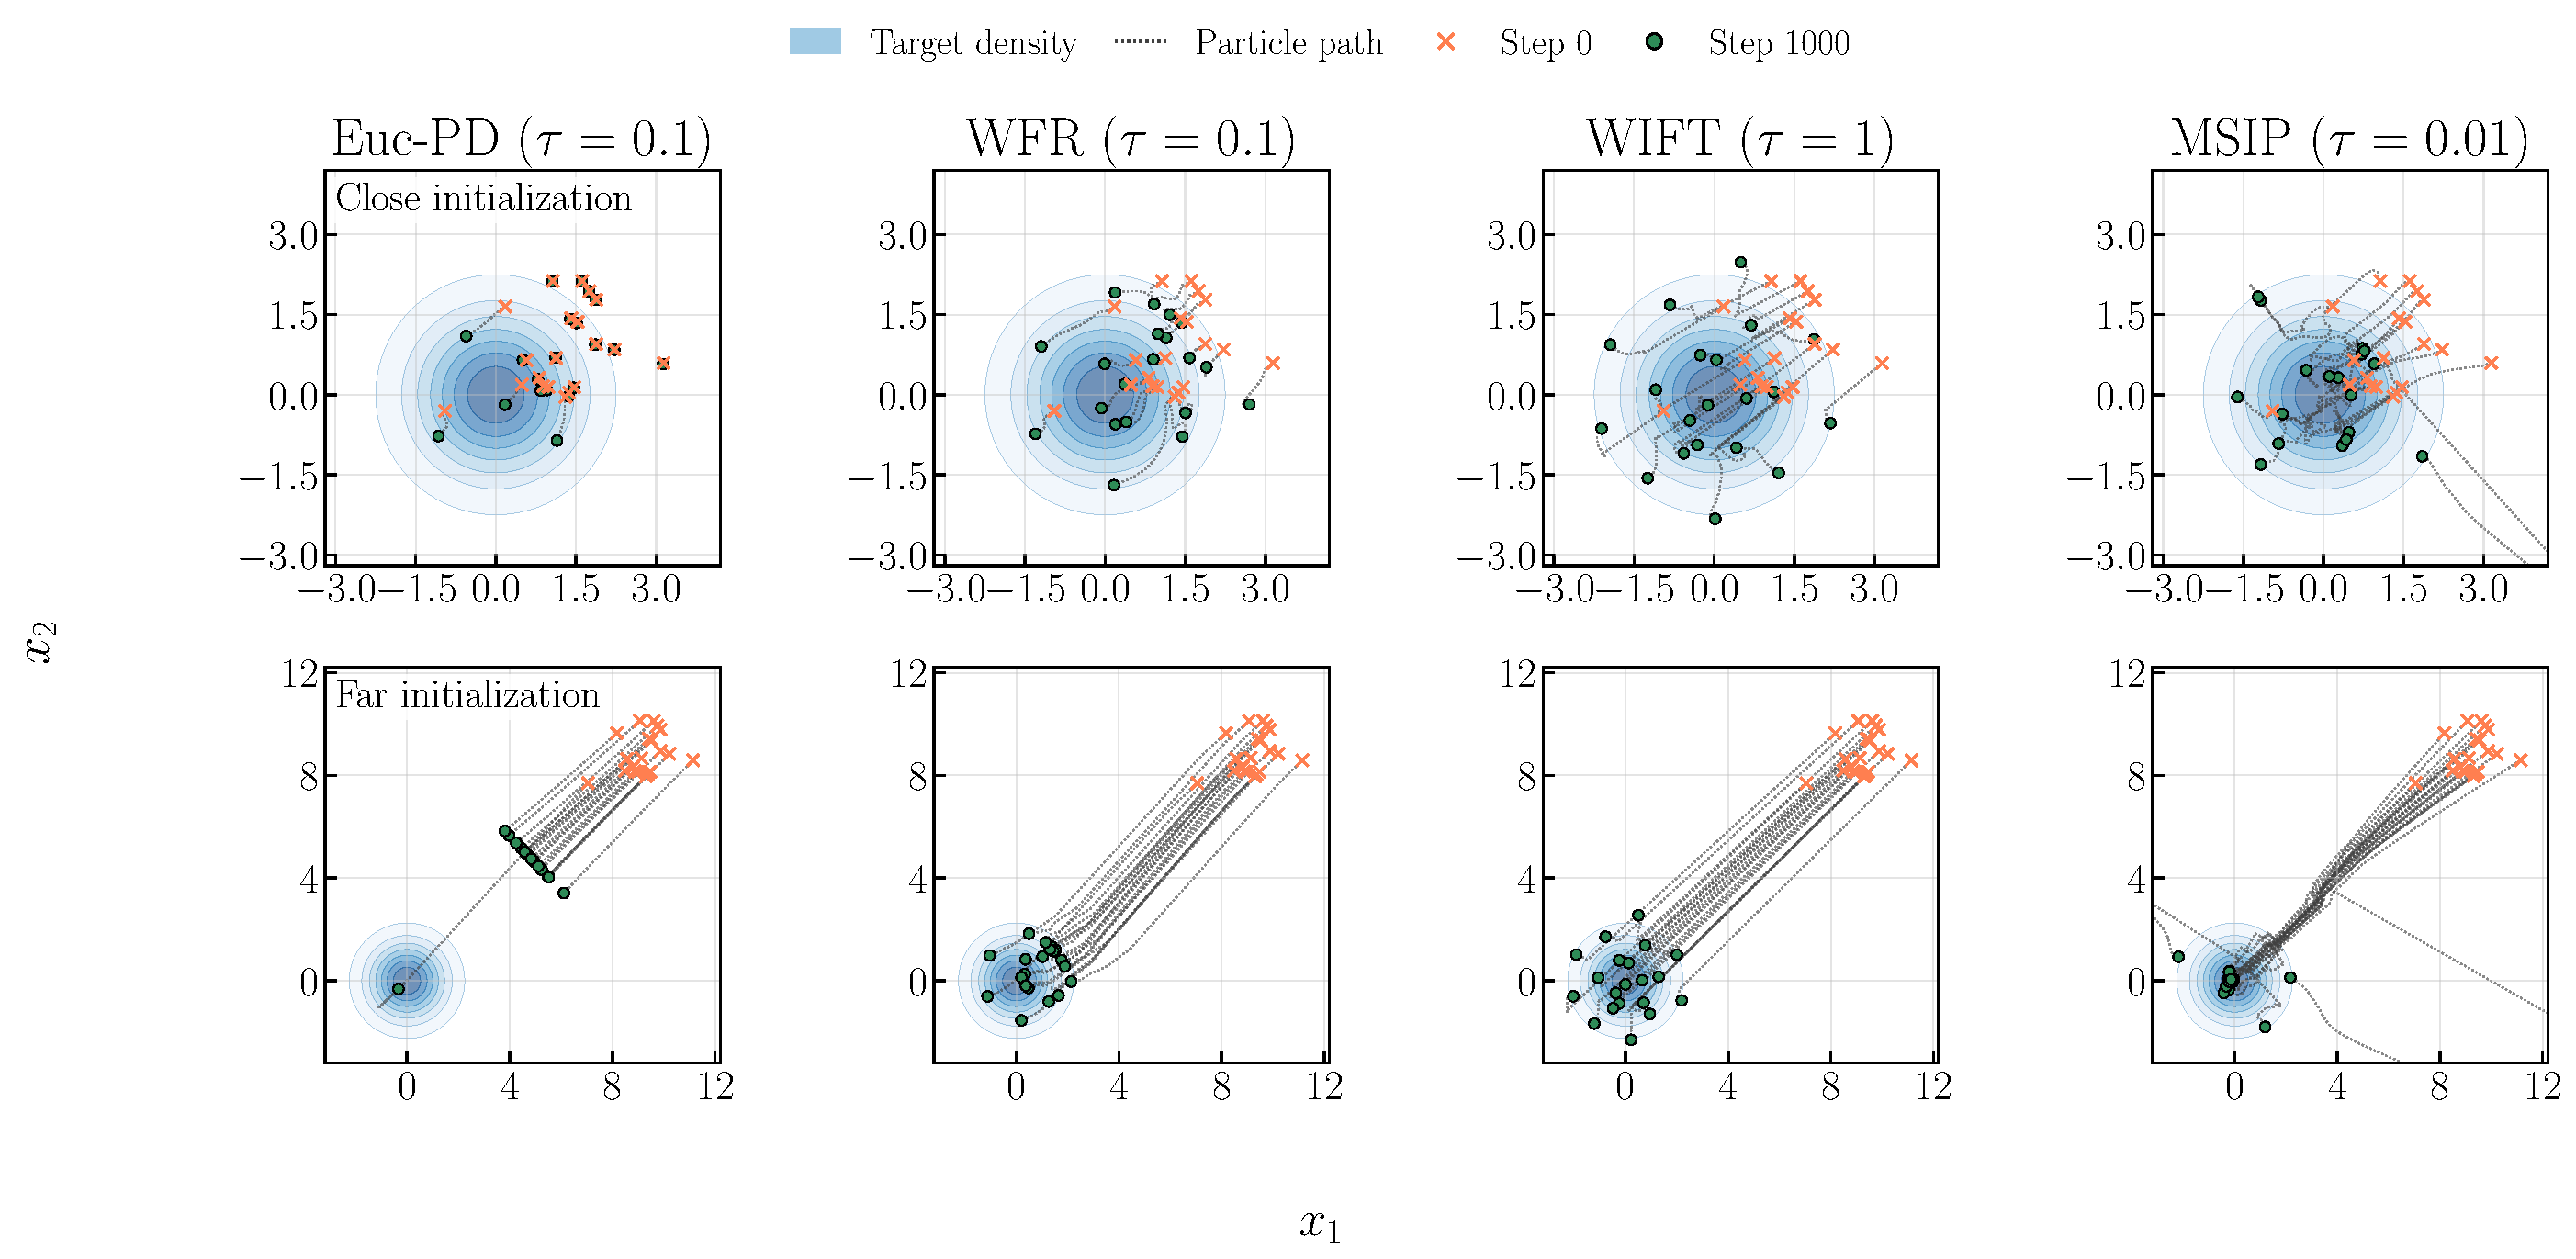
\includegraphics[width=1.0\linewidth]{figures/appendix_particle_trajectories.pdf}
    \caption{\textbf{Particle trajectories under close and far initialization.} Paths of all $20$ particles from step $0$ to step $1000$ for initial distributions $\mathcal{N}((1,1),I_2)$ and $\mathcal{N}((9,9),I_2)$, respectively.}
    \label{fig:appendix-particle-trajectories}
\end{figure}


% \newpage
% \input{include/checklist}

\end{document}
